\chapter{Methodology}
The methodology used in this research is based on the frameworks proposed by Asl et al. (2015) \cite{Asl2015}, Asl, A. and Wong, K. (2015) \cite{Asl2015a}, and Jiang, T. and Zhang, C. (2018) \cite{Jiang2018}. It is a mixture of the works of the aforementioned authors. In this chapter, we will first discuss about the mathematical model of the problem being solved. Later, we will be delving into the inner workings of the solution representation and then the algorithm.

\section{Mathematical Model}
The goal of any metaheuristic, like what is being proposed in this paper, is to optimize a certain objective function. As mentioned in the first chapter, in facility layout problems, we minimize the following function:

$$
\text{min} F = \sum_{i=1}^{n}\sum_{j=1}^{n}c_{ij}f_{ij}d_{ij}
$$

For the problem we are solving in this paper, we are optimizing the following equation that is not only a slight modifications of the basic mathematical model for FLPs, but also adds penalties to solutions that are infeasible, no matter the degree of infeasiblity.

\begin{align*}
	\text{min }F &= \sum_{i=1}^{\left | B \right |}\sum_{j=i + 1}^{\left | B \right |}c_{ij}d_{ij} \\
	& + \sum_{i=1}^{\left | B \right |}\sum_{j=i + 1}^{\left | B \right |} \left ( P_{B}\frac{A_{0}(i, j)}{\text{min}(w_{i}h_{i}, w_{j}h_{j})} + P_{B} \right ) \cdot \alpha_{0}(i, j) \\
	& + \sum_{i=1}^{\left | B \right |}\left( P_{R}\frac{w_{i}h_{i} - A_{1}(i)}{w_{i}h_{i}} + P_{R} \right) \cdot \alpha_{1}(i)
\end{align*}

where:

\begin{center}
	\begin{tabular}{| l | p{10cm} |}
	\hline
	$x_{i}$  & top-left $x$ coordinate of building $i$ \\
	\hline
	$y_{i}$  & top-left $y$ coordinate of building $i$ \\
	\hline
	$w_{i}$  & width of building $i$ \\
	\hline
	$h_{i}$  & height of building $i$ \\
	\hline
	$R_{x}$  & top-left $x$ coordinate of the bounding region \\
	\hline
	$R_{y}$  & top-left $y$ coordinate of the bounding region \\
	\hline
	$R_{w}$  & width of the bounding region \\
	\hline
	$R_{h}$  & height of the bounding region \\
	\hline
	$c_{ij}$ & flow rate from building $i$ to building $j$ \\
	\hline
	$d_{ij}$ & distance from the center of building $i$ to the
	           center of building $j$ \\
	\hline
	$P_{B}$  & penalty value for building intersection \\
	\hline
	$P_{T}$  & penalty value for any building going out of
	           bounds, even with a portion of a building \\
	\hline
	\end{tabular}
\end{center}

We elected to remove the flow rate from the basic formulation of the model that was discussed earlier in Equation \ref{mm-equation-mhc}. 

\begin{equation}\label{mm-equation-mhc}
	\sum_{i=1}^{\left | B \right |}\sum_{j=i + 1}^{\left | B \right |}c_{ij}d_{ij}
\end{equation}

This is because we can consider flow rate as simply part of cost. In the original formulation, we were considering it from a material handling cost perspective, which requires having both a cost and flow rate variable. However, in a general problem, we can consider cost to also include the frequency of movement from one facility to another, which is essentially the flow rate. As such, we can merge cost and flow rate into one variable.

The mathematical model allows for infeasible solutions to allow for better solutions in the long run. To follow this specification, the model includes expressions that penalizes solutions that meet any of the following conditions: (1) at least one building is intersecting with another building, and (2) a building, either in whole or in part, is outside the bounding area.

\begin{equation}\label{mm-equation-intersection}
	\sum_{i=1}^{\left | B \right |}\sum_{j=i + 1}^{\left | B \right |} \left ( P_{B}\frac{A_{0}(i, j)}{\text{min}(w_{i}h_{i}, w_{j}h_{j})} + P_{B} \right ) \cdot \alpha_{0}(i, j)
\end{equation}

Equation \ref{mm-equation-intersection} is the expression that applies a penalty to solutions that meet the first condition. Notice that it has the functions $A_{0}(i, j)$ and $\alpha_{0}(i, j)$. They are defined by the following:

\begin{align}
	A_{0}(i, j) &= I_{L}(x_{i}, x_{j}, w_{i}, w_{j})
	               \cdot I_{L}(y_{i}, y_{j}, h_{i}, h_{j}) \\
	I_{L}(x_{1}, x_{2}, l_{1}, l_{2}) &= \text{max}(0, \text{min}(x_{1} + l_{1}, x_{2} + l_{2}) - \text{max}(x_{1}, x_{2})) \\
    \alpha_{0}(i, j) &=
    \left\{\begin{matrix}
    	1 & \text{if } A_{0}(i, j) > 0 \\ 
    	0 & \text{otherwise}
    \end{matrix}\right.
\end{align}

$A_{0}(i, j)$ simply gets the area of intersection of buildings $i$ and $j$. This is achieved by the use of $I_{L}(x_{1}, x_{2}, l_{1}, l_{2})$, which computes the length or width of an intersection of buildings.

In the equation, for every pair of buildings that intersect, we apply a penalty that is the percentage of the area of the smallest building by area that is intersecting with the other building multiplied by the penalty value for building intersection. This will allow for rewarding the algorithm for moving the buildings towards non-intersection. The same penalty value is also added to ensure that the algorithm prioritizes removing intersections over reducing the distance between the centers of the buildings. $\alpha_{0}(i, j)$ ensures that the penalty is only applied to pairs of buildings that intersect with one another.

\begin{equation}\label{mm-equation-oob}
	\sum_{i=1}^{\left | B \right |}\left( P_{R}\frac{w_{i}h_{i} - A_{1}(i)}{w_{i}h_{i}} + P_{R} \right) \cdot \alpha_{1}(i)
\end{equation}

The other part of the mathematical model, Equation \ref{mm-equation-oob}, works in a similar principle as Equation \ref{mm-equation-intersection}. This equation applies a penalty value when the second condition of infeasibility is met. Like in \ref{mm-equation-intersection}, it has specific functions to help compute the penalty. They are defined as:

\begin{align}
	A_{1}(i) &= I_{L}(x_{i}, R_{x}, w_{i}, R_{w})
	\cdot I_{L}(y_{i}, R_{y}, h_{i}, R_{h}) \\
	\alpha_{1}(i) &=
	\left\{
	\begin{matrix}
		0 & \text{if} &
		\begin{aligned}
			R_{x} &\leq x_{i} &\leq R_{x} + R_{w} \\
			R_{x} &\leq x_{i} + w_{i} &\leq R_{x} + R_{w} \\
			R_{y} &\leq y_{i} &\leq R_{y} + R_{h} \\
			R_{y} &\leq y_{i} + h_{i} &\leq R_{y} + R_{h} \\
		\end{aligned} \\		
		1 & \text{otherwise}
	\end{matrix}\right.
\end{align}

$A_{1}(i)$ simply computes the area of intersection of the building and the bounding area. Now, since this only computes the intersection, we must subtract the intersection with the area of the building to get the area of the building that is outside of the bounding area. This is expressed by the numerator of the fractional expression in Equation \ref{mm-equation-oob}. Similar to Equation \ref{mm-equation-intersection}, the equation applies a penalty value that is the percentage of the area of the total building area that is outside the bounding region multiplied and then added by the penalty value. The addition is also to ensure that the algorithm gives more priority to removing out-of-bounds buildings. $\alpha_{1}(i)$ ensures that the penalty is only applied to buildings that are, in part or in whole, out of bounds.

\section{Solution Representation}
The solution is represented using a one-dimensional array of floating numbers. In the array, every group of three consecutive elements are considered to be the x and y positions, and angle, respectively, of one building. While the x and y positions are allowed to be of any value, the angle value is restricted to only $0^{\circ}$ and $90^{\circ}$. A visualization of the solution representation is shown by Figure \ref{solution-repr-viz}.

\begin{figure}
	\begin{center}
		\begin{tabular}{| c | c | c | c | c | c | c |}
			\hline
			$x_{0}$ & $y_{0}$ & $\angle_{0}$ & $\ddots$ & $x_{n - 1}$ & $y_{n - 1}$ & $\angle_{n - 1}$ \\
			\hline
		\end{tabular}
	\end{center}
	\caption{Visualization of the solution representation.}
	\label{solution-repr-viz}
\end{figure}

\section{The Algorithm}
\begin{figure}[c]
	\centering
	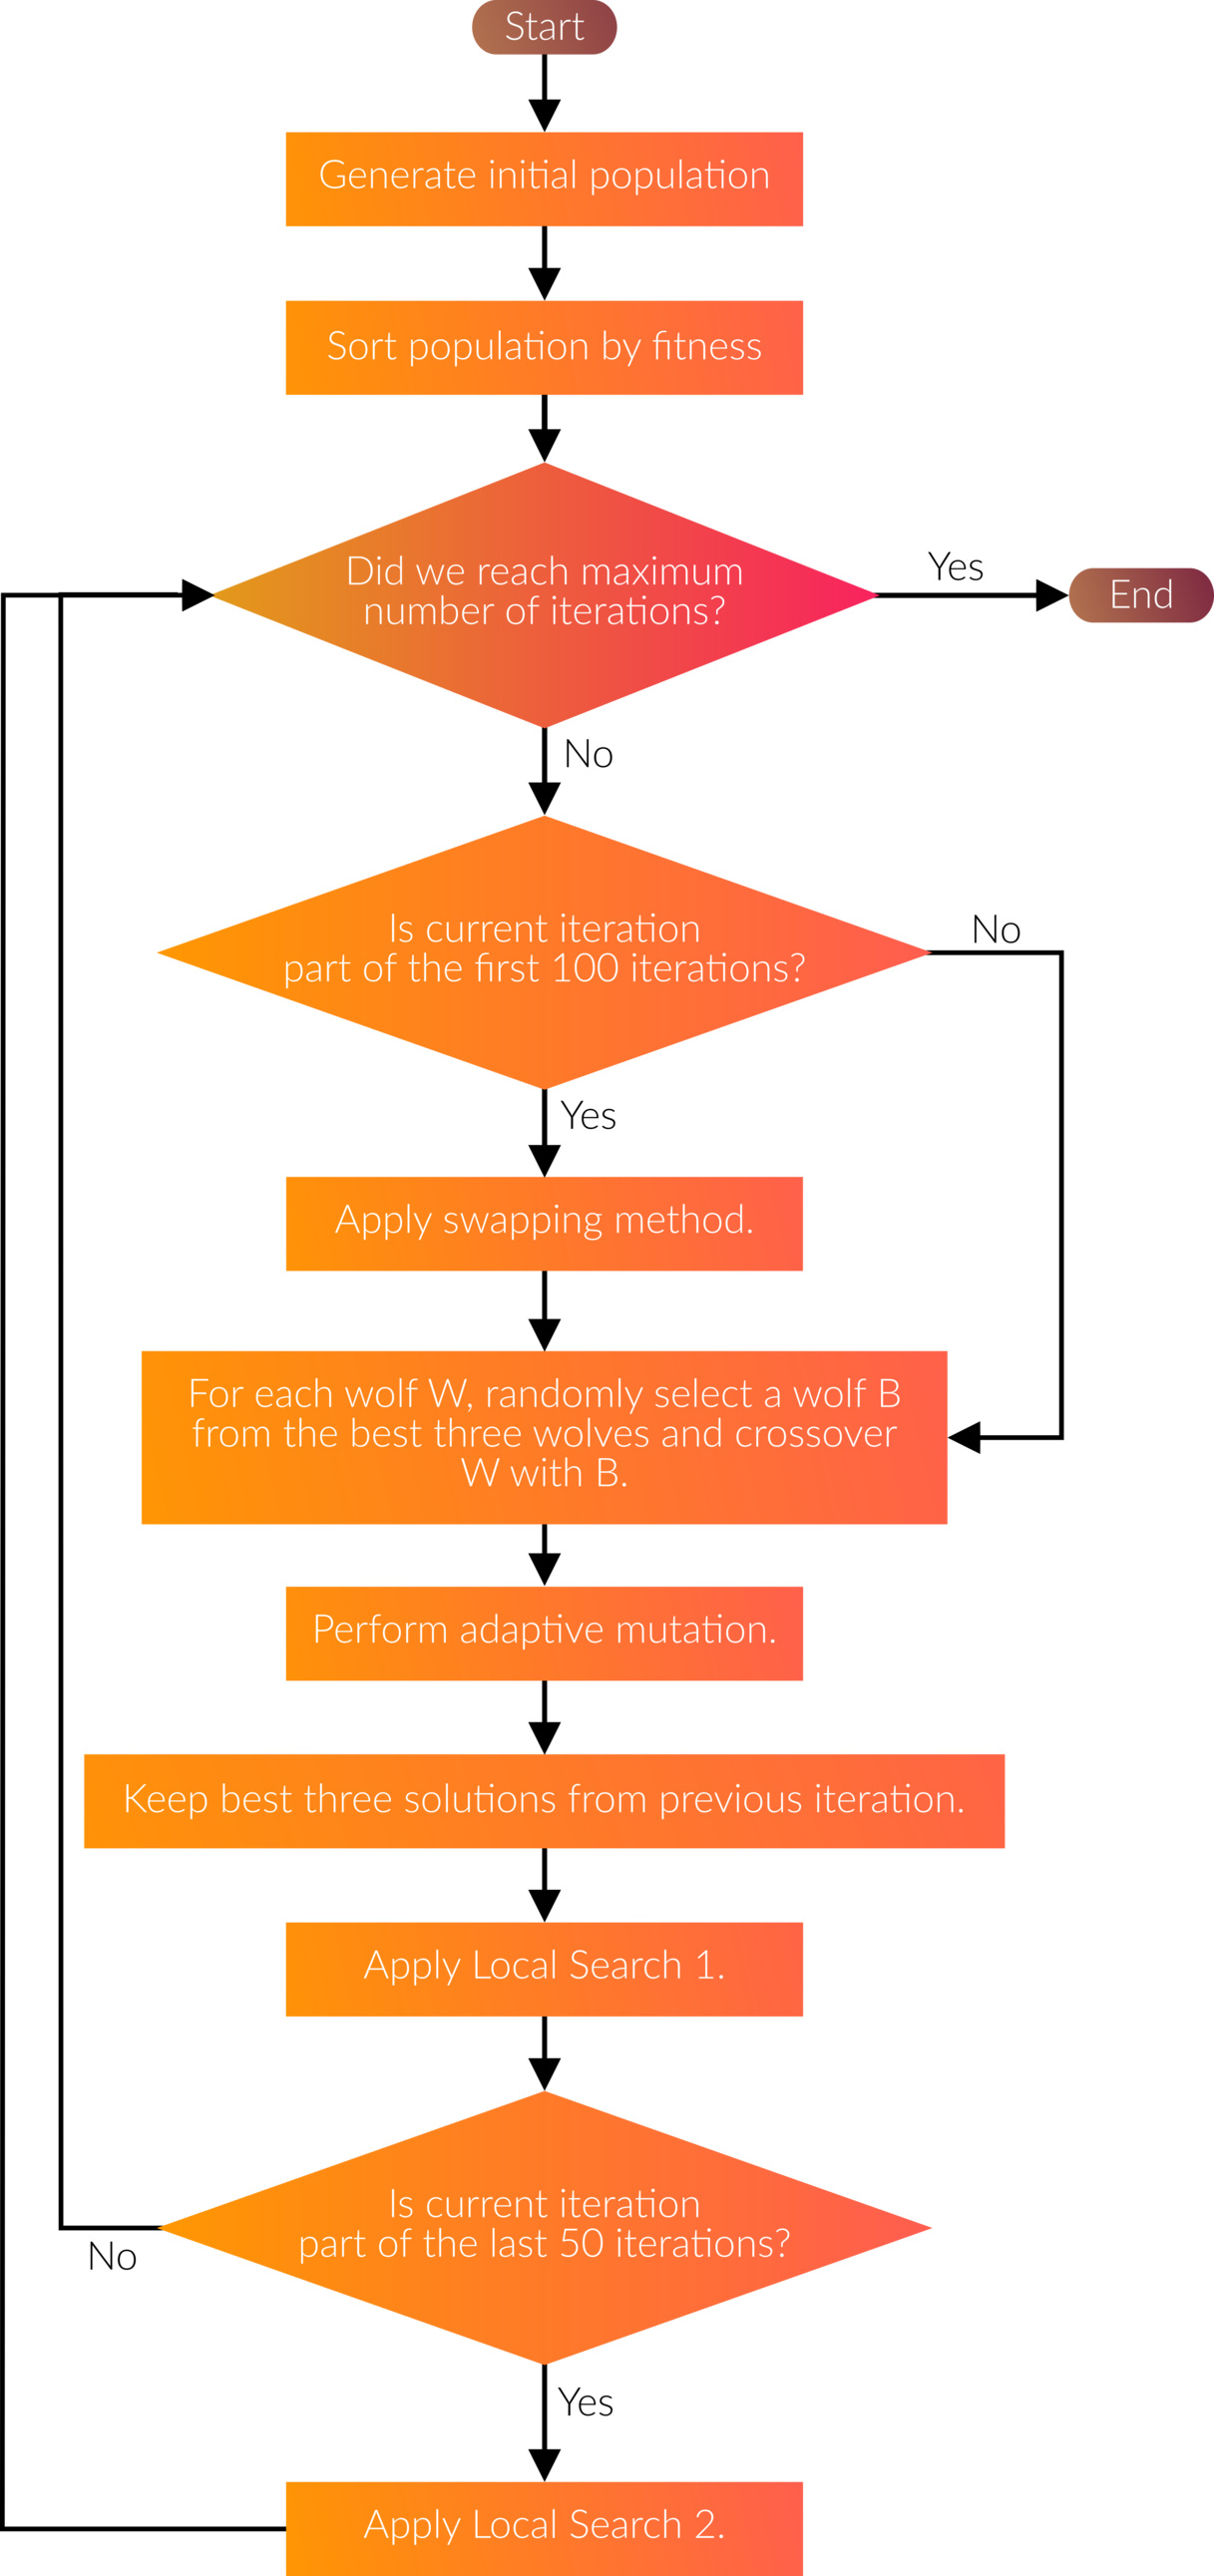
\includegraphics{./images/chap05-methodology/flowchart.png}
	\caption{Flowchart detailing the algorithm.}
	\label{algo-flowchart}
\end{figure}

The proposed algorithm contains multiple phases to solve the unequal area static facility layout problem. The basic framework of the algorithm is inspired from the works of Asl et al. (2015) \cite{Asl2015} and Asl, A. and Wong, K. (2015) \cite{Asl2015}. The Grey Wolf Optimization aspect of the algorithm is inspired from Jiang, T. and Zhang, C. (2018) \cite{Jiang2018}. Figure \ref{algo-flowchart} shows a flowchart of the algorithm. We will be further discussing the algorithm in detail in this section.

The advantage of this algorithm... // Continue this later.

\subsection{Population Generation}
In generating the initial population, the order in which facilities are placed in the bounding region is shuffled. Once it is shuffled, each building $i$ is then given a random x position between the inclusive range $\left [ R_{x} + \frac{w_{i}}{2}, (R_{x} + R_{w}) - \frac{w_{i}}{2} \right ]$, a random y position between the inclusive range $\left [ R_{y} + \frac{h_{i}}{2}, (R_{y} + R_{h})  - \frac{h_{i}}{2} \right ]$, and angle that is either $0^{\circ}$ or $90^{\circ}$ (chosen in a uniformly random fashion). This will generate a solution where the buildings are spread out throughout the bounding region. There will be building intersections (though this is dependent on the number of buildings and size of the bounding region), but no building will be out-of-bounds. This process is repeated until we generate a specified number of solutions. This number is determined by the population size.

\subsection{Swapping Method}
The swapping method is used to find a possible configuration for a solution that is better than the current configuration. This method is applied to all solutions in the population, but only in the first 100 iterations. Pseudocode for the swapping method is provided in Algorithm \ref{pseudocode-swapping}.

\begin{algorithm}
\caption{Pseudocode for the swapping method.}
\label{pseudocode-swapping}
\begin{algorithmic}[1]
\State Let $S$ be the collection of generated solutions.
\State Set $S_{curr}$ be the current solution.
\State Add $S_{curr}$ to $S$.
\State Set $N_{B}$ be the maximum number of buildings.
\For{i = 0 until $N_{B} - 2$}
	\For{j = i + 1 until $N_{B} - 1$}
		\State Building $i$'s orientation in $S_{curr}$ is changed to the other orientation,\WRP and the resulting new solution is added to $S$
		\State Building $j$'s orientation in $S_{curr}$ is changed to the other orientation,\WRP and the resulting new solution is added to $S$
		\State Building $i$'s and $j$'s orientations in $S_{curr}$ are changed to the other\WRP orientation, and the resulting new solution is added to $S$
		\State Building $i$'s and $j$'s positions are exchanged in $S_{curr}$, and the resulting new\WRP solutiA movement and a orientation changeon is added to $S$.
		\State Building $i$'s and $j$'s positions are exchanged in and the orientation of\WRP building $i$ is changed in $S_{curr}$, and the resulting new solution\WRP is added to $S$.
		\State Building $i$'s and $j$'s positions are exchanged in and the orientation of\WRP building $j$ is changed in $S_{curr}$, and the resulting new solution\WRP is added to $S$.
		\State Building $i$'s and $j$'s positions are exchanged in and the orientations of\WRP buildings $i$ and $j$ are changed in $S_{curr}$, and the resulting new solution\WRP is added to $S$.
	\EndFor
\EndFor \\
\Return the best solution in $S$.
\end{algorithmic}
\end{algorithm}

\subsection{Crossover, Mutation, and Elitism}
Experimentations with directly applying the formulas of Grey Wolf Optimization in solving our instance of the facility layout problem have not generated satisfying results. However, results generated by an algorithm inspired from the paper of Jiang, T., and Zhang, C. (2018) \cite{Jiang2018} showed promise. As such the GWO portion of our proposed approach has been taken from their work. Their work takes certain elements from genetic algorithms, particularly the crossover and mutation operators, but kept the general principle of Grey Wolf optimization intact. We will be discussing each operator in detail in this section. Elitism is also implemented in our proposed approach to ensure that the best solutions found so far do not get lost throughout iterations. It will also be discussed in this section.

\subsubsection{Crossover}
Grey wolf optimization algorithms breed with the other solutions with the top three solutions in the population. That is modelled by the mathematical definition of the optimization algorithm. However, directly the definition does not yield good results. Due to that, we are using a crossover operator from the work of Jiang, T., and Zhang, C. (2018) \cite{Jiang2018}.

The crossover operator used here can be mathematical defined as:

$$
X(t + 1) =
\begin{cases}
	f(X(t), X_{alpha}(t)) & \text{if }
	\text{rnd} \leq \frac{1}{3} \\ 
	f(X(t), X_{beta}(t)) & \text{if }
	\frac{1}{3} < \text{rnd} \leq \frac{2}{3} \\
	f(X(t), X_{delta}(t)) & \text{if }
	\text{rnd} \geq \frac{2}{3}
\end{cases} 
$$

where $f$ is the crossover function, and $\text{rnd} \sim U(0, 1)$. This means that a solution will be crossed over by one of the best three solutions, selected randomly. In our approach, we have used the uniform crossover. Note that this crossover is applied to every solution in a population in accordance with the principle of GWO. In our approach, only one offspring is generated from the crossover.

\subsubsection{Mutation}
Over time, as more and more iterations are performed, the diversity of the population will eventually be lost. This is due to the fact that the wolves are only updated based on the best three solutions. This will also result in premature convergence \cite{Jiang2018}. To combat this, a mutation operator is performed to reintroduce diversity. The mutation operator used is an operator that we dub the "Buddy-Buddy Mutation".

The \textbf{Buddy-Buddy Mutation} is a mutation operator that simply selects two pairs of buildings $D$ and $S$, and move one of them to the side of the other building. Building $D$ is referred to as the dynamic buddy, while building $S$ is referred to as the static buddy. Building $D$ will be the building that will be moved towards the other building, which is building $S$ in our case. When moving building $D$, a side $E$ of building $S$ will first be randomly chosen. Afterwards, an orientation for building $D$ will be randomly chosen, whether it will be parallel or perpendicular to $E$. Once a side and orientation has been selected, building $D$ will be moved adjacent towards building $S$ at side $E$ with the chosen orientation. The implementation of this mutation operator in our proposed approach gives buildings that intersect with another building more chances of being selected as the dynamic buddy. Pseudocode and a visualization of the operator is provided by Algorithm \ref{pseudocode-buddybuddy-mutation} and Figure \ref{buddy-buddy-mutation-viz}, respectively.

\begin{algorithm}
	\caption{Pseudocode for the Buddy-Buddy Mutation.}
	\label{pseudocode-buddybuddy-mutation}
	\begin{algorithmic}[1]
		\State Randomly select two buildings $D$ and $S$, with more weight given to buildings that are intersecting with another.
		\State Set $E$ to be a randomly selected side of building $S$.
		\State Set $O$ to either be a parallel or perpendicular orientation, randomly selected.
		\State Move building $D$ adjacent to side $E$ of building $S$ with the orientation $O$.
	\end{algorithmic}
\end{algorithm}

The rate at which a solution is mutated is highly dependent on the fitness of the solution. The worse the fitness of a solution is, the more likely it is to be mutated. This encourages the proposed algorithm to improve solutions that are generally bad. This rate scheme makes this an adaptive mutation operator \cite{Jiang2018}. The mutation rate is mathematically modelled as:

\begin{equation}
	m(X, t) = 1 - \frac{fit_{max}(t) - fit(X(t))}{fit_{max}(t) - fit_{min}(t)}
\end{equation}

where $m_{k}$ refers to the mutation rate of a solution $X$ at iteration $t$, $fit$ is a function that gets the fitness of a solution, and $fit_{min}$ and $fit_{max}$ gets the minimum and maximum fitnesses of the population, respectively.

\subsubsection{Elitism}
One variant of genetic algorithms includes elitism. This elitism allows a genetic algorithm to keep a number of best solutions in the next generation, ensuring that the best solutions do not get discarded over time. Note that this elitism strategy is not only limited to genetic algorithms. Other evolutionary algorithms may also utilize this strategy \cite{Du2018}. We are also taking this principle into our proposed approach. In our proposed approach, we are keeping the best three solutions in the previous iteration to the next iteration. We chose three due to the fact that the best three solutions in a population have significance in GWO.

\subsection{Local Searches}
Remember that our implementation is based on aforementioned previous works that used local search algorithms in conjunction to genetic algorithms. They combined GAs with local search algorithms because GAs find it hard to explore within the convergence area. Hybridizing it with a local search algorithm improves performance \cite{Ripon2013}. In our proposed approach, we are keeping this aspect of the previous works. This will also ensure that we are able to search within the convergence area more intensely and find better solutions. In the previous works and in ours, there are two local search algorithms, dubbed "Local Search 1" and "Local Search 2". They vary in terms of searching intensity, but both attempts to obtain better solutions. We will be discussing details of both in this section.

\subsubsection{Local Search 1}
The first local search algorithm, "Local Search 1", performs a local search by creating a number of solutions by moving each building in different directions by a certain random amount and changing its orientations after movement and obtaining the best solution from these activities. In our approach, the certain amount of movement is a random number between 1 and 5. This search algorithm is only applied to the best solution of the current iteration, and the best solution found in this search becomes the new best solution and replaces the previously best solution. The movements of each building is defined by a set of "activities". This set of activities is shown by Table \cite{local-search-1-activities}. Additionally, a pseudocode of the search algorithm is shown in Algorithm \ref{pseudocode-local-search-1}.

\begin{figure}
	\begin{center}
		\begin{tabular}{| c | p{110mm} |}
			\hline
			Activity Number & Description \\
			\hline
			0 & A building is moved to the right along the x-axis by a random number between 1 and 5. \\
			1 & A building is moved to the left along the x-axis by a random number between 1 and 5. \\
			2 & A building is moved to the upwards along the y-axis by a random number between 1 and 5. \\
			3 & A building is moved to the downwards along the y-axis by a random number between 1 and 5. \\
			4 & Generate two random numbers from 1 and 5 and a building is moved to the right and then upward, respectively, by those numbers. \\
			5 & Generate two random numbers from 1 and 5 and a building is moved to the right and then downward, respectively, by those numbers. \\
			6 & Generate two random numbers from 1 and 5 and a building is moved to the left and then upward, respectively, by those numbers. \\
			7 & Generate two random numbers from 1 and 5 and a building is moved to the left and then downward, respectively, by those numbers. \\
			\hline
		\end{tabular}
	\end{center}
	\caption{Activities for moving a building in Local Search 1}
	\label{local-search-1-activities}
\end{figure}

\begin{algorithm}
\caption{Pseudocode for Local Search 1.}
\label{pseudocode-local-search-1}
\begin{algorithmic}[1]
\State Set $S$ to be a collection of solutions.
\State Set $S_{curr}$ to be the solution being optimized.
\State Add $S_{curr}$ to $S$.
\State Set $N_{B}$ be the maximum number of buildings.
\State Set $N_{A}$ be the maximum number of activities.
\For{i = 0 until $N_{B} - 1$}
	\For{a = 0 until $N_{B} - 1$}
		\State Perform activity $a$ with building $i$ in $S_{curr}$ and save the new solution in $S$.
		\State Perform activity $a$ with building $i$, and change the orientation of the building to the other orientation in $S_{curr}$ and save the new solution in $S$.
	\EndFor
\EndFor \\
\Return the best solution in $S$.
\end{algorithmic}
\end{algorithm}

\subsubsection{Local Search 2}
Local Search 2 is a more intense version of Local Search 1, in order to find the best solution so far. Unlike the latter that only moves one building at a time, Local Search 2 moves two buildings instead. The two buildings will also have their orientations changed after each activity. This local search is only applied to the best solution found in the last 50 iterations. The set of activities for this local search is shown by Table \cite{local-search-2-activities}, and a pseudocode of the search algorithm is shown in Algorithm \ref{pseudocode-local-search-2}.

\begin{figure}
	\begin{center}
		\begin{tabular}{| c | p{110mm} |}
			\hline
			Activity Number & Description \\
			\hline
			0  & Building $i$ and $i + 1$ are moved to the right along the x-axis by a random number between 1 and 5. \\
			1  & Building $i$ and $i + 1$ are moved to the left along the x-axis by a random number between 1 and 5. \\
			2  & Building $i$ and $i + 1$ are moved upwards along the x-axis by a random number between 1 and 5. \\
			3  & Building $i$ and $i + 1$ are moved downwards along the x-axis by a random number between 1 and 5. \\
			4  & Generate two random numbers from 1 and 5 and buildings $i$ and $i + 1$ are moved to the right and then upward, respectively, by those numbers. \\
			5  & Generate two random numbers from 1 and 5 and buildings $i$ and $i + 1$ are moved to the right and then downward, respectively, by those numbers. \\
			6  & Generate two random numbers from 1 and 5 and buildings $i$ and $i + 1$ are moved to the left and then upward, respectively, by those numbers. \\
			7  & Generate two random numbers from 1 and 5 and buildings $i$ and $i + 1$ are moved to the left and then downward, respectively, by those numbers. \\
			8  & Generate two random numbers $a$ and $b$ that are from 1 to 5, and building $i$ is moved upward by $a$ and building $i + 1$ is moved to the right by $b$. \\
			9  & Generate two random numbers $a$ and $b$ that are from 1 to 5, and building $i$ is moved upward by $a$ and building $i + 1$ is moved downward by $b$. \\
			10 & Generate two random numbers $a$ and $b$ that are from 1 to 5, and building $i$ is moved upward by $a$ and building $i + 1$ is moved to the left by $b$. \\
			11 & Generate two random numbers $a$ and $b$ that are from 1 to 5, and building $i$ is moved to the right by $a$ and building $i + 1$ is moved downward by $b$. \\
			12 & Generate two random numbers $a$ and $b$ that are from 1 to 5, and building $i$ is moved to the right by $a$ and building $i + 1$ is moved upward by $b$. \\
			13 & Generate two random numbers $a$ and $b$ that are from 1 to 5, and building $i$ is moved to the right by $a$ and building $i + 1$ is moved to the left by $b$. \\
			14 & Generate two random numbers $a$ and $b$ that are from 1 to 5, and building $i$ is moved to the left by $a$ and building $i + 1$ is moved to downward by $b$. \\
			15 & Generate two random numbers $a$ and $b$ that are from 1 to 5, and building $i$ is moved to the left by $a$ and building $i + 1$ is moved to the right by $b$. \\
			16 & Generate two random numbers $a$ and $b$ that are from 1 to 5, and building $i$ is moved to the left by $a$ and building $i + 1$ is moved upward by $b$. \\
			17 & Generate two random numbers $a$ and $b$ that are from 1 to 5, and building $i$ is moved downward by $a$ and building $i + 1$ is moved to the right by $b$. \\
			18 & Generate two random numbers $a$ and $b$ that are from 1 to 5, and building $i$ is moved downward by $a$ and building $i + 1$ is moved to the left by $b$. \\
			19 & Generate two random numbers $a$ and $b$ that are from 1 to 5, and building $i$ is moved downward by $a$ and building $i + 1$ is moved upward by $b$. \\
			\hline
		\end{tabular}
	\end{center}
	\caption{Activities for moving a building in Local Search 2}
	\label{local-search-2-activities}
\end{figure}

\begin{algorithm}
	\caption{Pseudocode for Local Search 2.}
	\label{pseudocode-local-search-2}
	\begin{algorithmic}[1]
		\State Set $S$ to be a collection of solutions.
		\State Set $S_{curr}$ to be the solution being optimized.
		\State Add $S_{curr}$ to $S$.
		\State Set $N_{B}$ be the maximum number of buildings.
		\State Set $N_{A}$ be the maximum number of activities.
		\For{i = 0 until $N_{B} - 2$}
		\For{a = 0 until $N_{B} - 1$}
		\State Perform activity $a$ with building $i$ in $S_{curr}$ and save the new solution in $S$.
		\State Perform activity $a$ with building $i$, and change the orientation of \WRP building $i$ to the other orientation in $S_{curr}$ and save the new \WRP solution in $S$.
		\State Perform activity $a$ with building $i$, and change the orientation of \WRP building $i + 1$ to the other orientation in $S_{curr}$ and save the new \WRP solution in $S$.
		\State Perform activity $a$ with building $i$, and change the orientations of \WRP buildings $i$ and $i + 1$ to the other orientations in $S_{curr}$ and save the new \WRP solution in $S$.
		\EndFor
		\EndFor \\
		\Return the best solution in $S$.
	\end{algorithmic}
\end{algorithm}